\section{Results}
\section{Instances}
\color{green} Would move it to a testing section right before evaluation \color{black}\\
sparse\_0\_1 means sparse with 0\% malfunctions the first one.
\color{blue}
\begin{itemize}
	\item would make it a testing section
	\item explain instances (why how, ...)
	\item explain benchmarking (how, why, ...)
\end{itemize}
\color{black}

\subsection{Sparse instances}

\begin{figure}	
	\begin{minipage}{.41\textwidth}
		\begin{subfigure}{\textwidth}
			\centering
			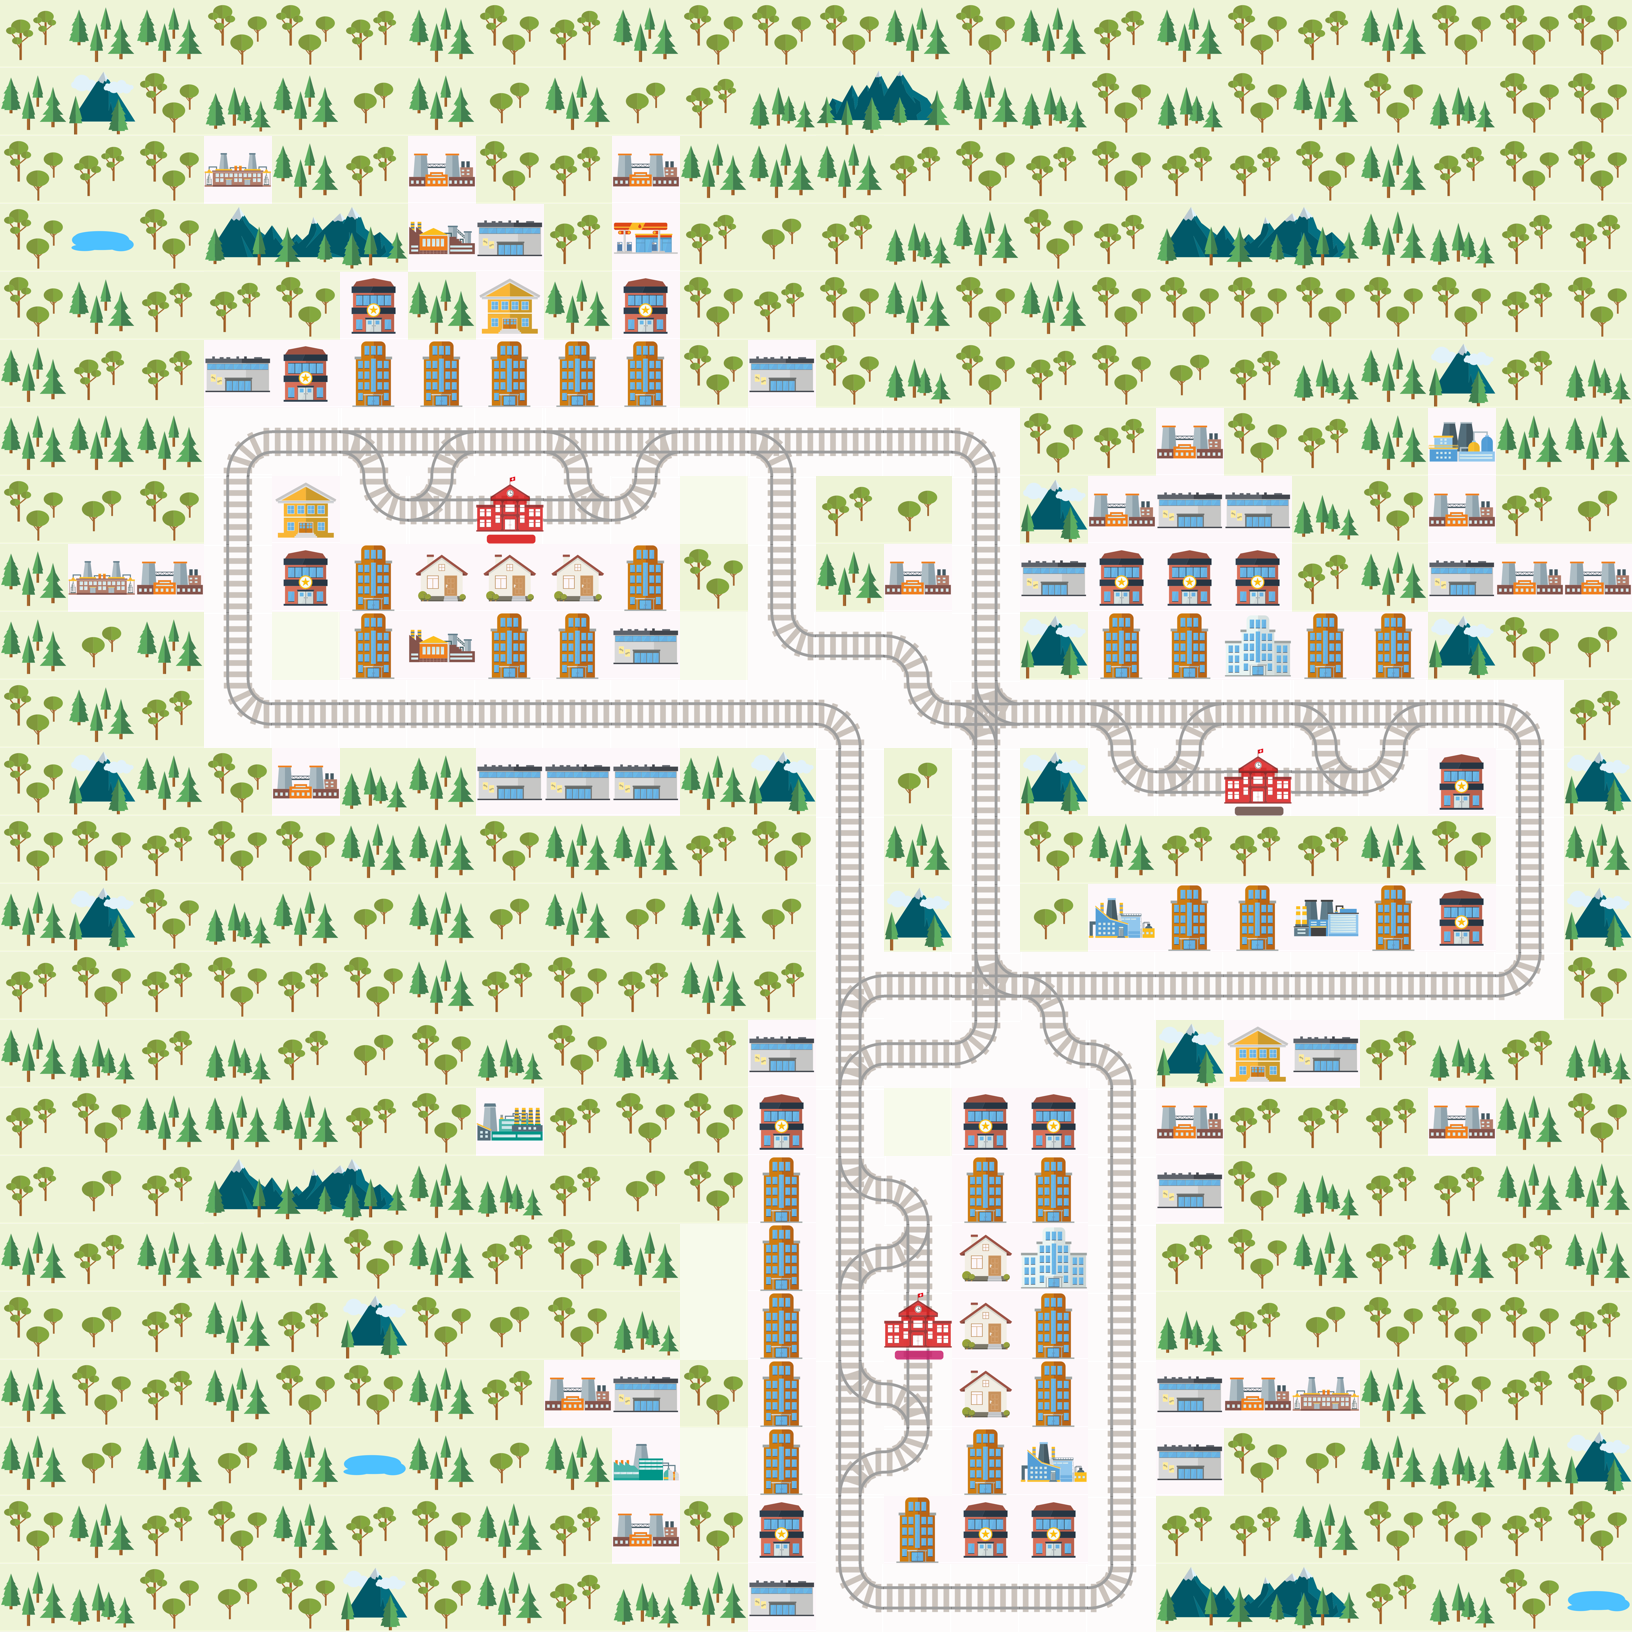
\includegraphics[width=0.48\textwidth]{dense/dense_0_1}
			\caption{Dense instance, using a 24x24 grid, where 20 trains must travel across 3 cities.}
			\label{dense_0_1}
		\end{subfigure}
	\hfill
		\begin{subfigure}{\textwidth}
			\centering
			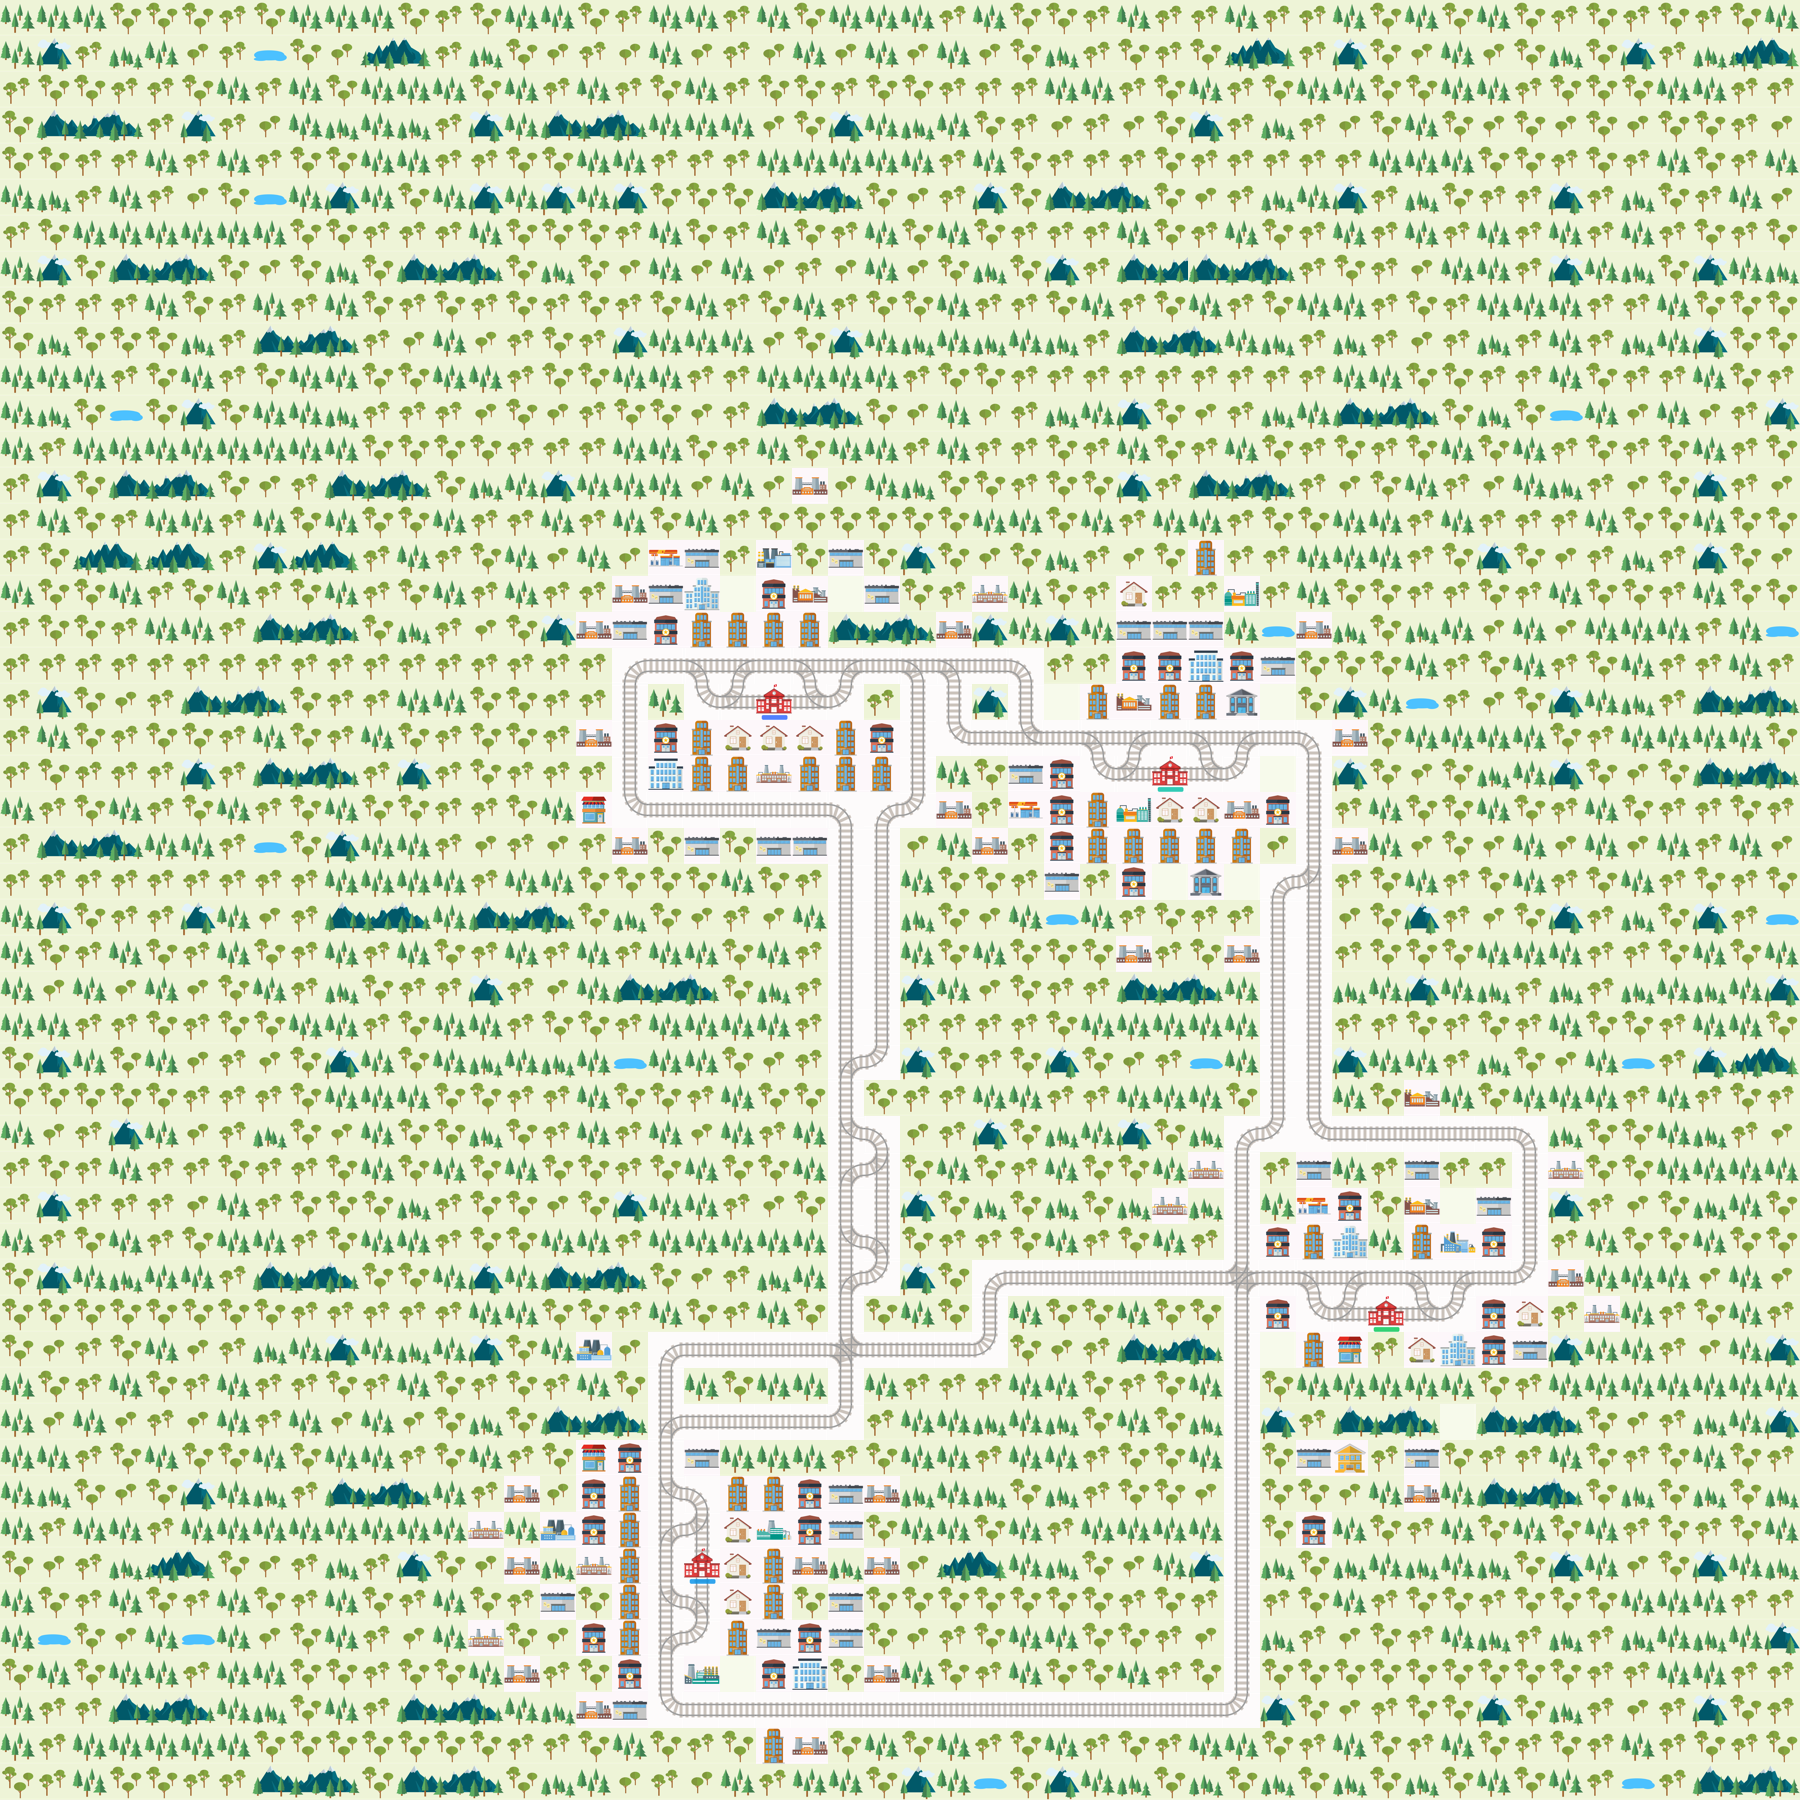
\includegraphics[width=\textwidth]{medium/medium_0_1}
			\caption{Medium instance, using a 50x50 grid, where 10 trains must travel across 5 cities.}
			\label{medium_0_1}
		\end{subfigure}
	\end{minipage}
	\hfill
	\begin{minipage}{.49\textwidth}
				\begin{subfigure}{\textwidth}
		\centering
		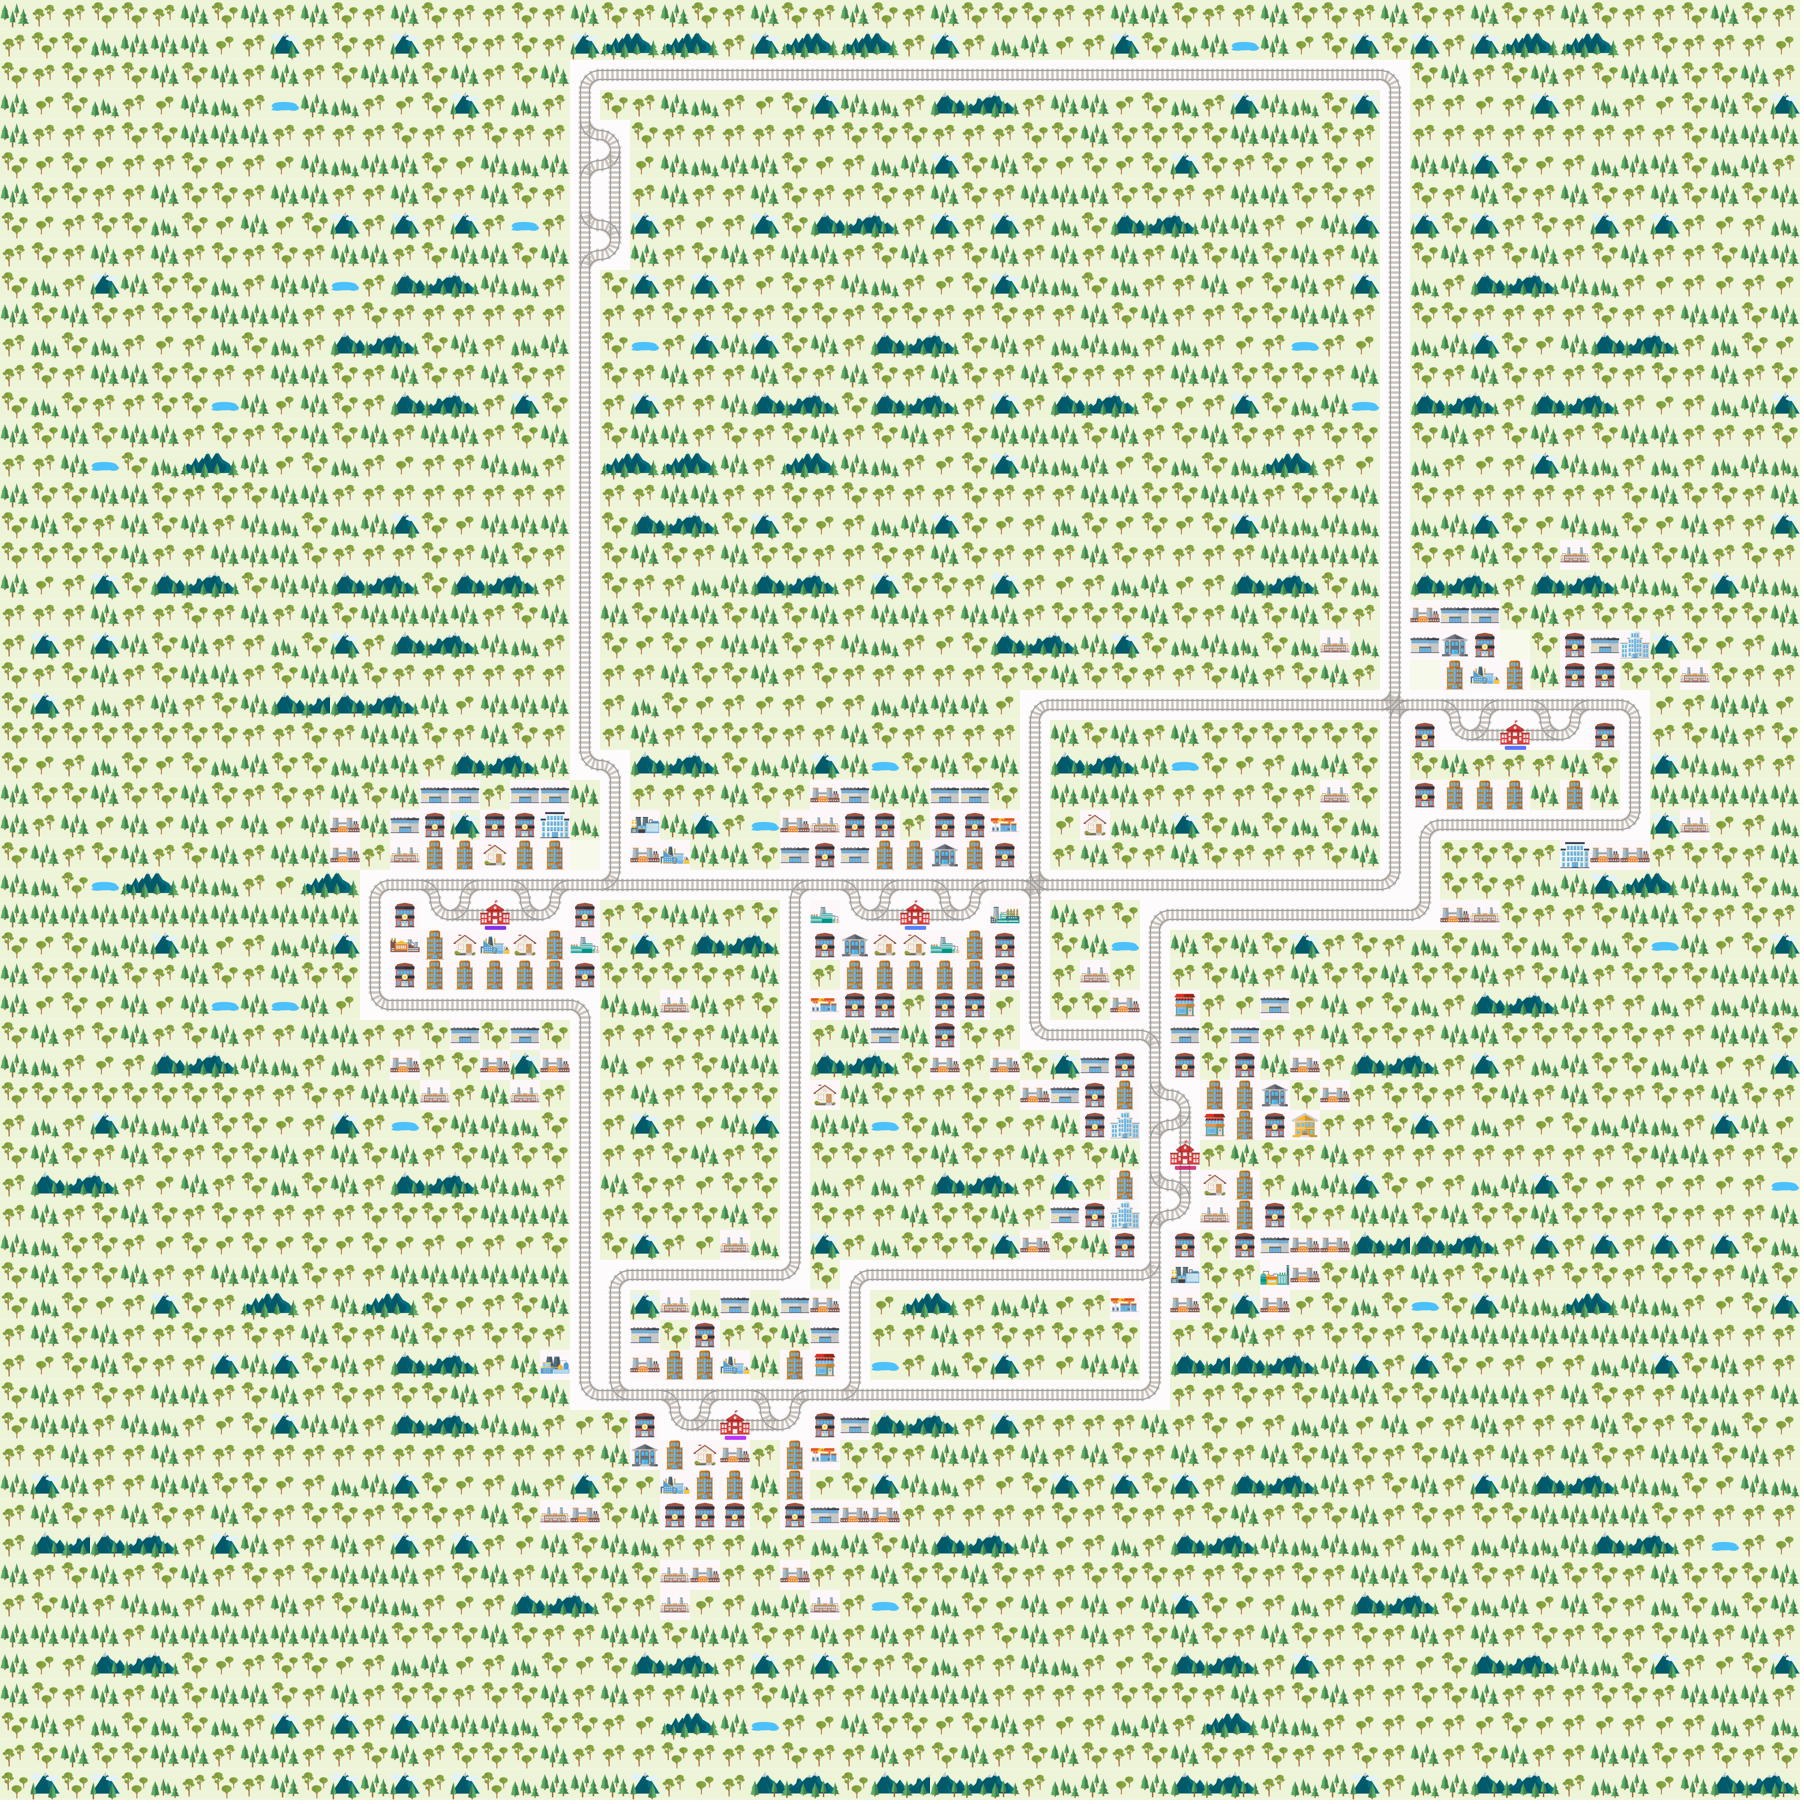
\includegraphics[width=\textwidth]{sparse/sparse_0_1}
		\caption{Sparse instance, using a 60x60 grid, where 6 trains must travel across 6 cities.}
		\label{sparse_0_1}
				\end{subfigure}
	\end{minipage}
	\caption{The 3 types of configurations used for our experimentation, put side-by-side in order to get an idea of the scale. The full list can be found at \cite{instance_folder}}
	\label{sparse_medium_dense}
\end{figure}

\subsection{Medium instances}

\subsection{Dense instances}